\section{Overview}
\label{sec:overview}

We now walk through an 
  example
  of how current FPGA technology mapping tools can fail
  a hardware designer (\cref{sec:overview-part-1}) 
  and how \lr overcomes these limitations (\cref{sec:overview-part-2}).
In the process,
  we provide a high-level overview
  of \lr's main components.

\subsection{Compiling a Design to a DSP with Existing Tools}
\label{sec:overview-part-1}

Consider the following scenario:
A hardware designer
  is designing a large hardware block
  for the Xilinx UltraScale+ family of FPGAs.
The designer is specifically aiming to use 
  the UltraScale+'s specialized DSP48E2 units,
  which 
  can implement 
  combined multiplication, arithmetic,
  and logic operations, as 
  captured in this 
  simplified
  block diagram~\cite{userguide}:
\begin{center}
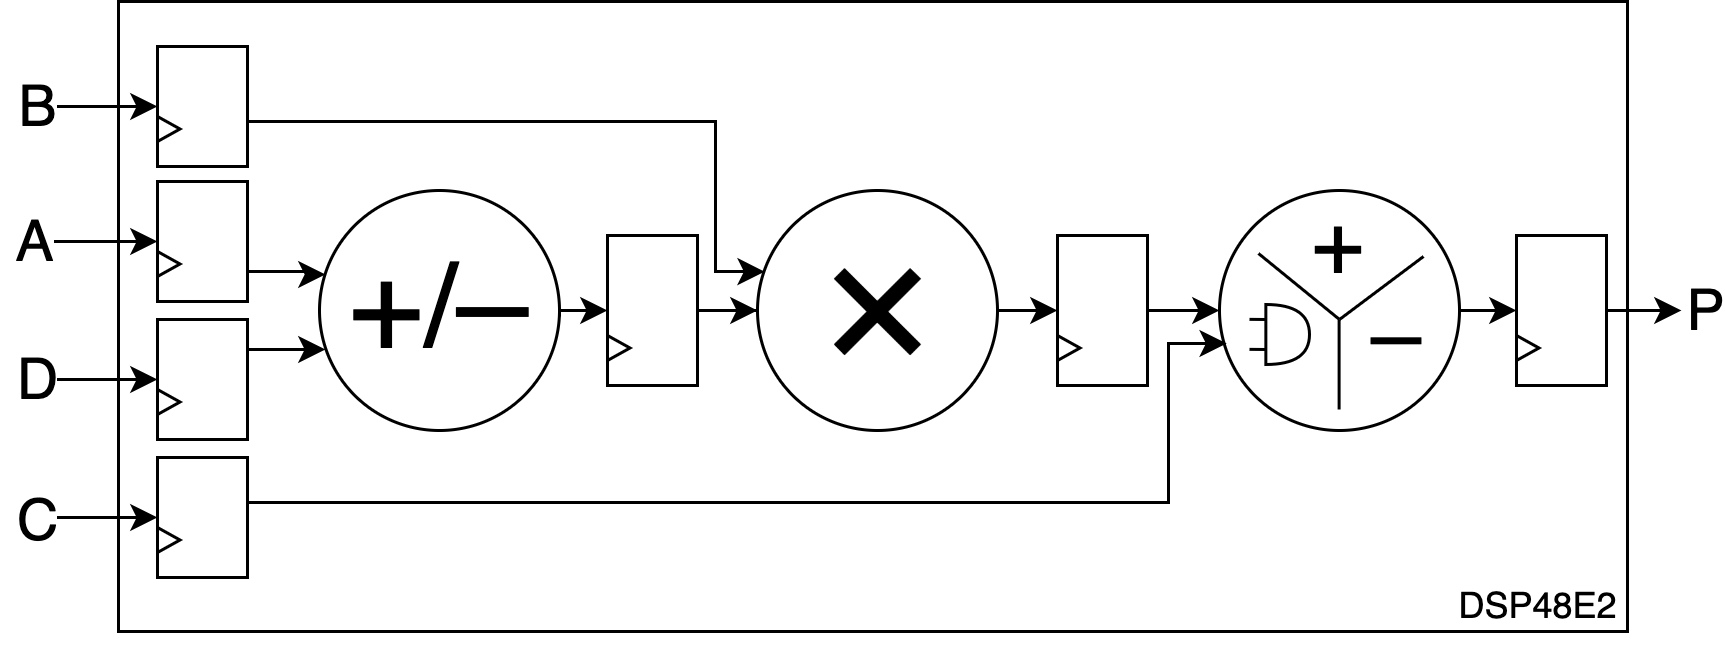
\includegraphics[width=.75\columnwidth]{lakeroad/assets/dsp48e2-block-diagram-simplified.drawio.png}
\end{center}
The designer's hardware block
  involves the computation
  \texttt{(c-a)*b},
  which the manual states is implementable with a single DSP.
%Specifically, imagine their design
%involves the following computation, 
  %applied
  %four separate times:
In particular, suppose the design
  consists of four separate instances of the following computation:
\begin{center}
\begin{minted}[baselinestretch=1]{verilog}
 for(i=0; i<4; i++) begin
  r[i] <= (c[i] - a[i]) * b[i];
 end
\end{minted}
\end{center}
%Thus, the designer expects that this design
  %should fit on a total of
  %four DSPs.
It would be reasonable for the designer
  to expect the design
  to use a total of four DSPs.

\textit{\textbf{Current tools fail.}}
After compiling the design
  with existing tools,
  the designer is frustrated
  to find that the compiler returns a design
  that uses more
  resources than anticipated.
Instead of using the expected
  four DSPs, it uses eight---%
  a 100\% increase in resource consumption!
\textbf{The compiler has thus failed to 
  fully utilize
  the DSP}---%
  it has not configured a DSP48E2
  to implement
  \texttt{(c-a)*b} but has instead
  overflowed the
  computation
  onto
  an extra DSP.
The designer now faces a choice:
  either accept the result or attempt to coax the compiler
  into returning a more optimal design.

\textit{\textbf{Coaxing the compiler, to no avail.}}
Though many 
may choose to accept a less optimal result,
 this tenacious designer\footnote{
This may not be purely a personal preference. %of a tenacious designer.
%that go down this path.
For example, a hardware design simply may not fit on an FPGA
  without manual optimizations!}
  tries to coax
  the compiler into giving the 
  expected results
  by 
  placing the computation
  of interest into a separate module:

\begin{minted}[baselinestretch=1]{verilog}
module sub_mul(input clk, input [15:0] a, b, c,
                   output reg [15:0] out);
 assign out = (c-a)*b;
endmodule
\end{minted}

\noindent
This allows the designer
  to  apply
  %extra effort and
  specific optimizations while mapping
  the module---%
  a process we call \textit{partial design mapping}.
They attempt various strategies,
  including
  annotating the module with
  Xilinx's \texttt{use\_dsp} Verilog attribute
  (to force the compiler to use a DSP where possible)
  and using a different
  synthesis directive
  (to apply a more 
  resource-intensive synthesis
  procedure).
\textbf{Despite these efforts,
  the compiler still cannot 
  map the design
  to a single DSP,}
  instead using two DSPs
  for the partial design.
Again, the designer must decide:
  give up and accept
  suboptimal results,
  or press on?

\textit{\textbf{Manual compilation.}}
The hardware designer presses on and
  % having failed to coax the compiler
  % into mapping the
  % \texttt{sub\_mul} module to a single
  now has only one option remaining:
  manually instantiating a DSP48E2
  with the desired behavior.
Skimming through the daunting 75-page DSP48E2's online user manual,
  the designer quickly discovers that
  configuring even
  the ``pre-sub'' \texttt{c-a}
  requires correctly setting 
  multiple ports and parameters
  (\texttt{INMODE}, \texttt{AMULTSEL}, \texttt{BMULTSEL}, and \texttt{PREADDINSEL}),
  whose descriptions span 10+ pages and multiple tables.
Correctly configuring the subsequent multiplier
  and logic unit proves even more difficult
  and time-consuming.
After configuring the computational units,
  the designer must still manually ensure
  correct pipelining
  of the 10+ pipeline registers.
After hours
  of frustration,
  a configuration is found that 
  seems to work, which the designer
  inserts into the design.
Precious time has been wasted,
  most of which will need to be repeated
  to configure the DSP again.
Making matters worse,
  \textbf{the designer has no formal guarantees
  about the correctness of this DSP configuration.}
It may work in a few simulated test cases,
  but are there corner cases
  that have been missed?\tighten

%\textit{What next?}
%\sandy{I think you can omit the next 3 sentences since the points have already been succinctly made and go directly to sentence 4 ("Next, we examine..."}

%\textit{\textbf{Summary.}}
%The designer, disappointed
  %by state-of-the-art compilers,  
  %was forced to
  %manually configure a DSP,
  %costing hours to days of effort.
%To boot, there are 
  %no guarantees that
  %the final configuration is correct.
%Next, we examine how \lr
  %saves time and effort
  %while also guaranteeing correctness.

  
\subsection{Compiling a Design to a DSP with \lr}
\label{sec:overview-part-2}

\lr can save hardware designers
  the great effort involved
  in manual DSP configuration
  while also providing correctness guarantees.
Let us imagine how the designer 
  in this example,
  frustrated by conventional tools,
  can instead proceed using \lr
  during partial design mapping.
%Frustrated by conventional tools,
  %let's now imagine the designer
  %chooses to use \lr
  %during partial design mapping.
After putting 
  \texttt{sub\_mul}
  into its own module,
  the designer calls
  \lr from the command line:
\begin{minted}[baselinestretch=1]{bash}
$ lakeroad --template dsp \
           --arch-desc xilinx-ultrascale-plus.yml \
           sub_mul.v
\end{minted}
% (Note that we have excluded some flags for this example.)
The \texttt{lakeroad} command outputs
  \texttt{sub\_mul\_impl},
  an implementation
  of \texttt{sub\_mul}
  that uses a single UltraScale+ DSP48E2:
\begin{minted}[baselinestretch=1]{verilog}
module sub_mul_impl(input clk, input [15:0] a, b, c, output [15:0] out);
 DSP48E2 #(
  .ACASCREG(32'd0), .ADREG(32'd0), .ALUMODEREG(32'd0),
  .AMULTSEL("AD"), .AREG(32'd0), .AUTORESET_PATDET("NO_RESET"), 
  // ...plus 30+ more parameters
 ) DSP48E2_0 (
   .A({ 14'h0000, a }), .ACIN(30'h00000000), .ALUMODE(4'hc),
   .B({ 2'h0, b }), .BCIN(18'h00000), .C({ 32'h00000000, c }),
   .CARRYCASCIN(1'h0), .CARRYIN(1'h0), .CARRYINSEL(3'h6),
   // ...plus 30+ more ports
 );
endmodule
\end{minted}
%
Unlike current compilers,
  \lr has produced an implementation
  using a single DSP48E2
  by utilizing more of the DSP's features.
Importantly, this compiled design
  is also formally guaranteed
  to implement
  the input \texttt{sub\_mul}
  design.
  
% \begin{wrapfigure}{r}{.5\textwidth}
\begin{figure}
    \centering
    \hspace{-1cm}%
    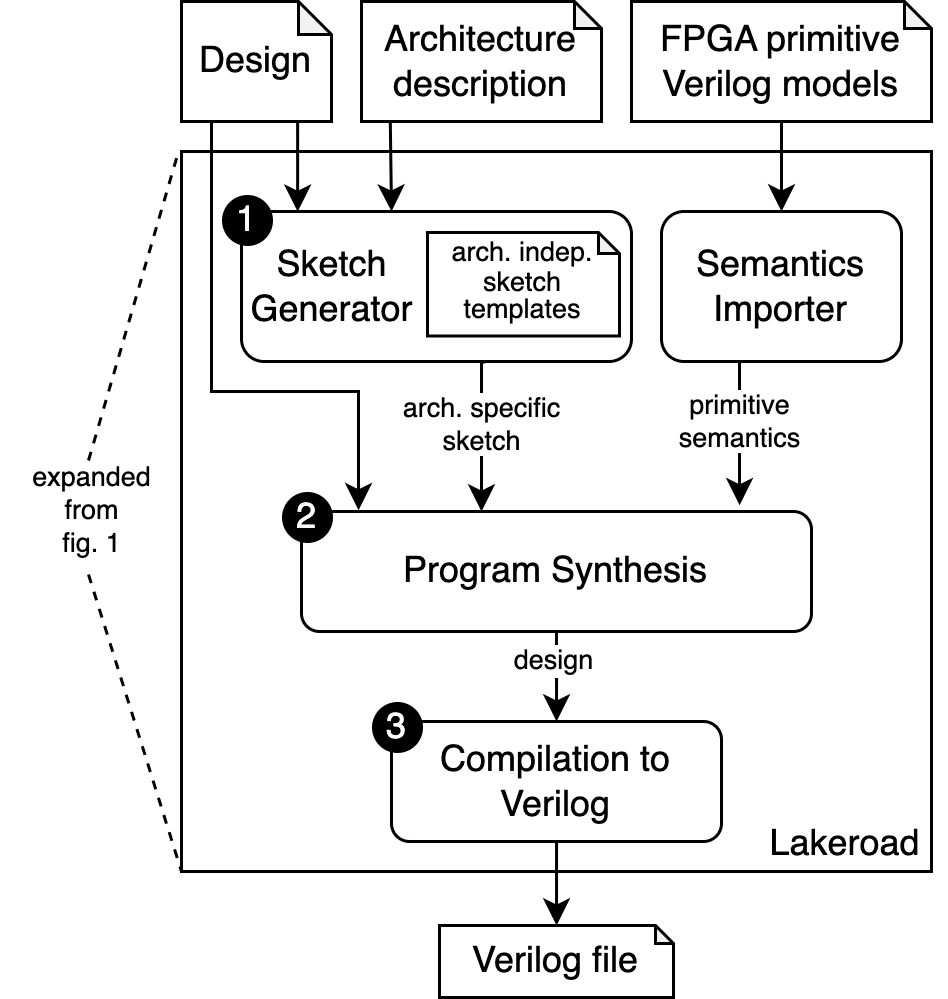
\includegraphics[width=.5\columnwidth]{lakeroad/assets/lakeroad-diagram.drawio.png}
   \caption{The components within \lr.}
    \label{fig:lakeroad-diagram}
\end{figure}
% \end{wrapfigure}

How does \lr provide 
  \textit{verified, more complete} support
  for the DSP48E2 over existing tools?  
At the core of \lr's
  correctness and completeness
  is
  \textit{sketch-guided program synthesis},
  a technique that  
  begins with a program \textit{sketch}, which
  captures a rough
  outline of a program
  and uses
  automated reasoning tools
  (e.g., SMT solvers)
  to fill in the sketch's \textit{holes.}
As shown in \cref{fig:lakeroad-diagram}, 
  \lr uses the following three-step process  
  to generate an efficient and correct
  DSP48E2 implementation
  of
  the \texttt{sub\_mul}
  design.
%This walkthrough follows the steps laid out visually in \cref{fig:lakeroad-diagram}. We begin by describing how \lr generates sketches.

\textit{\textbf{Step 1: Generating a Sketch.}}
In
  the \texttt{sub\_mul}
  example,
  \lr
  generates
  the following sketch,
  which we refer to as \texttt{sketch}:\footnote{
Though this example is presented in a Verilog-like language,
  \lr's sketches are actually encoded in a Racket DSL that resembles structural Verilog.
  }
% \begin{minipage}{\textwidth} % To prevent breaking the code across pages
\begin{minted}[baselinestretch=1]{verilog}
module sketch(input clk, input [15:0] a, b, c, output [15:0] out);
 DSP48E2 #(
  .ACASCREG(??), .ADREG(??), .ALUMODEREG(??), .AMULTSEL(??), 
  .AREG(??), .AUTORESET_PATDET(??), ...
 ) DSP48E2_0 (
   .A({ 14'h0000, a }), .ACIN(??), .ALUMODE(??), 
   .B({ 2'h0, b }), .BCIN(??), .C({ 32'h00000000, c }),
   .CARRYCASCIN(??),  .CARRYIN(??), .CARRYINSEL(??), ...
 );
endmodule
\end{minted}
  % \end{minipage}
\noindent
This sketch consists of a single DSP48E2 instance
  with \textit{holes} 
  (represented by \texttt{??}) 
  serving as placeholders for most of its ports and parameters.
It is easy to see  
  the parallels
  between \texttt{sketch}
  and
  \texttt{sub\_mul\_impl};
  \texttt{sketch}
  is simply 
  \texttt{sub\_mul\_impl}
  with holes.
But how does \lr generate \texttt{sketch}
  in the first place?

To maximize portability across architectures,
  \lr does not store sketches 
  like \texttt{sketch}
  directly; 
  instead, it \textit{generates} sketches
  from architecture-independent
  \textbf{sketch templates.}
Instead of storing
  the preceding UltraScale+--specific sketch,
  \lr generates the sketch
  from the DSP sketch template, which
  the designer has chosen to use 
  with the \mbox{\texttt{-{}-template dsp}} flag.
A simplified form of this template looks like the following:
\begin{minted}[baselinestretch=1]{verilog}
module dsp_sketch_template(input clk,
                           input [n-1:0] a, b, c,
                           output [n-1:0] out);
 DSP dsp_instance(.clk(clk), .A(a), .B(b), .C(c), .D(d), .out(out));
endmodule
\end{minted}
Sketch templates
  capture hardware design patterns
that are common across FPGA architectures
  in an
  architecture-independent way.
\texttt{dsp\_sketch\_template},
  for example, 
  captures
  a basic pattern, i.e., 
  instantiating a single DSP.
\lr includes 
  sketch templates of varying complexity,
  from the simplicity of the one above 
  to the complexity of LUT-based multipliers.
Though new sketch templates
  can be added easily,
  in most cases
  (as in this example)
  users can simply apply
  \lr's provided templates.

To specialize \texttt{dsp\_sketch\_template}
  into \texttt{sketch},
  \lr translates
  the sketch template's generic \texttt{DSP}
  \textbf{primitive interface}
  into an UltraScale+--specific
  DSP48E2
  using the UltraScale+
  \textbf{architecture description.}
The generic \texttt{DSP}
  module is an instance of a
  \textbf{primitive interface:} 
  a \lr-introduced abstraction that 
  %is generic across its parameters and
  captures the similarities
  between primitives across 
  diverse FPGA architectures.
For example, 
  \lr's DSP primitive interface
  captures the facts that
  DSPs on all FPGA platforms
  generally have two to four data inputs
  (captured by \texttt{A}--\texttt{D};
  note that our example doesn't use
  input \texttt{D})
  and a clock input
  (captured by \texttt{clk}).
To convert the
  sketch template's
  DSP primitive interface instance
  into a DSP48E2,
  \lr utilizes the
  Xilinx UltraScale+ architecture description,
  which the designer has pointed to with the 
  \texttt{-{}-arch-desc xilinx-ultrascale-plus.yml}
  flag.
An \textbf{architecture description}
  specifies how \lr's various
  primitive interfaces
  are implemented for a given architecture.
The following simplified snippet of the UltraScale+
  architecture description, for example,
  tells \lr that,
  when generating a sketch for 
  UltraScale+,
  instances of the DSP
  primitive interface
  should be implemented with a DSP48E2:
\begin{minted}[baselinestretch=1]{yaml}
- interface: {name: DSP, params: { out-width: 48, a-width: 30, ...}} 
  holes: [?ACASCREG, ?ADREG, ?ALUMODEREG, ?AREG, ...]
  implementation:
    module: DSP48E2
    ports: [{ name: A, bitwidth: 30, value: A }, ...]
    parameters: [{ name: ACASCREG, value: ?ACASCREG }, ...]
    outputs: { O : P }
\end{minted}
Thus, while converting
  \texttt{dsp\_sketch\_template}
  into
  \texttt{sketch},
  \lr reads this architecture description
  and converts the single DSP instance
  into a DSP48E2,
  filling the ports and parameters with the concrete values
  and holes
  contained in the architecture description.
Architecture descriptions
  are usually short (100-400 LoC)
  and
  written only once per FPGA architecture; 
  \lr already contains such descriptions
  for Xilinx UltraScale+,
  Xilinx 7-series,
  Lattice ECP5,
  Intel Cyclone 10 LP,
  and the open-source FPGA SOFA~\cite{sofa}.
%   Removed the below because
%     we don't really know what platforms
%     "real" users of Lakeroad
%     are going to need.
%   Unless we have a compelling reason
%   to believe that the platforms
%   above are the "correct" list,
%   I don't think we should say this.
%   --Steve
%Most \lr users
  %will not need to write their own
  %architecture descriptions.

To generate a sketch,
  \lr takes an architecture-independent
  sketch template
  and specializes it using an
  architecture description.
Once the sketch is ready,
  the designer can move on to synthesis.

\textit{\textbf{Step 2: Program Synthesis.}}
  The next step 
  %requires the designer to fill 
  fills
  in the holes to generate
  a complete, correct
  hardware design,
  which is done automatically
  using a technique called
  \gls{program-synthesis}.
\textit{Program synthesis} is the process of
  using automated reasoning tools
  (like \gls{smt} solvers) 
  to generate correct programs
  by encoding program generation
  as a constraint solving problem.
In our \texttt{sub\_mul} example,
  \lr, aided  by
  Rosette~\cite{torlak2013growing,torlak2014lightweight}, 
  generates a query like the following:\footnote{
  We formalize this synthesis query and explain it precisely in \cref{sec:formalization}.
}
\footnotesize
$$\exists \ \mathtt{ACASCREG}, \mathtt{ADREG}, ...\ .\ \forall \ \mathrm{inputs} . \ 
  \texttt{sub\_mul}(\mathrm{inputs}) 
  = \texttt{sketch}(\mathrm{inputs}, \mathtt{ACASCREG}, \mathtt{ADREG}, ...)
$$
\normalsize
The query asks:
  are there concrete values for
  \texttt{ACASCREG}, \texttt{ADREG}, etc.,
  that will make our sketch's behavior
  equivalent to the input design's behavior
  on all inputs?
If the solver finds such values,
  %\sandy{Note that the use of "we" creates uncertainty about who is doing what....the designer? Lakeroad? Please read and clarify.}
\lr can use them to fill the holes
  in the sketch
  and produce a compiled design.
However, if \lr tries to pass the preceding formula
  to an SMT solver,
  the solver will throw an error since
  the query is not expressed
  at a level 
 it understands, viz., %
  as equalities
  between bitvector expressions,
  using simple Boolean or arithmetic
  operations.
While it is conceivable that \texttt{sub\_mul}
  could be converted to
  a bitvector expression
  since its core computation is already
  expressed as
  \texttt{(c-a)*b},
it is unclear how to express
  \texttt{sketch}
  as an expression over bitvectors.
In particular, \lr must express
  bitvector-level semantics
  for Xilinx's DSP48E2 primitive.
%Specifically, where does \lr get bitvector-level
  %semantics
  %for Xilinx's DSP48E2 primitive?

To generate bitvector-level semantics
  for complex FPGA primitives,
  \lr introduces the concept of
  \textbf{semantics extraction}.
Rather than requiring
  manual effort to encode the semantics
  of the underlying hardware,
  which is notoriously difficult
  even for experts~\cite{Bernstein2021WhatAT},
  \lr's key insight is that these challenges
  can be avoided altogether
  by extracting low-level semantics
  directly from
  vendor-supplied simulation and verification models.
  % s provide models of their
  % primitives for simulation and verification,
  % such as Xilinx's \texttt{DSP48E2.v}
  % included with Vivado, Xilinx's proprietary
  % hardware synthesis tool.
\lr builds on internal passes in 
  Yosys~\cite{wolf2013yosys} 
  to automatically extract
  solver-ready semantics from these vendor-provided HDL models,
  which we detail in \cref{sec:implementation:importing-semantics}.
For the
  \texttt{sub\_mul} example,
  the DSP48E2's semantics have already been imported into \lr.
Semantics need to be imported only when
  adding support for a new architecture, i.e., %
  about as infrequently
  as writing a new architecture description.
In most cases,
  \lr users can rely on already-imported semantics.
  
With the sketch generated
  and the DSP48E2's semantics imported,
  program synthesis can begin.
\lr utilizes Rosette to drive program synthesis,
  as detailed in \cref{sec:formalization}.
In our example, Rosette returns
  a configuration for the DSP48E2.
The last step, then, is to convert
  the compiled design
  to Verilog.
  
\textit{\textbf{Step 3: Compilation to Verilog.}}
%Once program synthesis finds a valid assignment
  %of the holes in \texttt{sketch},
%\lr fills in the holes
  %to produce a concrete hardware design.
%In the last step, the designer compiles 
  %\lr's internal representation
  %into Verilog.
Compiling \lr's internal representation into Verilog
  is a purely 
  one-to-one syntactic mapping;
  no optimizations are done at this stage,
  reducing the likelihood that bugs could be inserted.
In our example,
  the final Verilog produced
  results in the
  \texttt{sub\_mul\_impl}
  we saw at the start of \cref{sec:overview-part-2}.

\textit{\textbf{In summary.}}
\lr
  delivered 
  an implementation
  of the designer's
  \texttt{sub\_mul}
  module,
  improving upon both state-of-the-art compilers
  and manual approaches
  in multiple ways.
\lr's implementation
  is significantly more resource-efficient
  than the state-of-the-art compiler's.
\lr delivered its implementation
  in mere seconds,
  compared to the hours to days
  of work
  that manually instantiating
  a DSP might take.
Lastly,
  \lr's implementation
  is formally guaranteed to be correct.
Meanwhile, \lr did all of this
  while requiring no input from the user
  other than the Verilog to be compiled.

In the next chapter,
  we provide details on the concepts introduced in this overview.
We begin by formalizing \lr's compilation flow in \cref{sec:formalization}, 
  covering sketches and program synthesis in detail.
Then, in \cref{sec:implementation}, we give implementation details for sketch templates, primitive interfaces, semantics importing, and compilation to Verilog.
  

